
\section*{Supplementary Methods: The \zcor Algorithm}
\def\ICD{ICD10\xspace}

\begin{wrapfigure}[26]{l}{4in}

  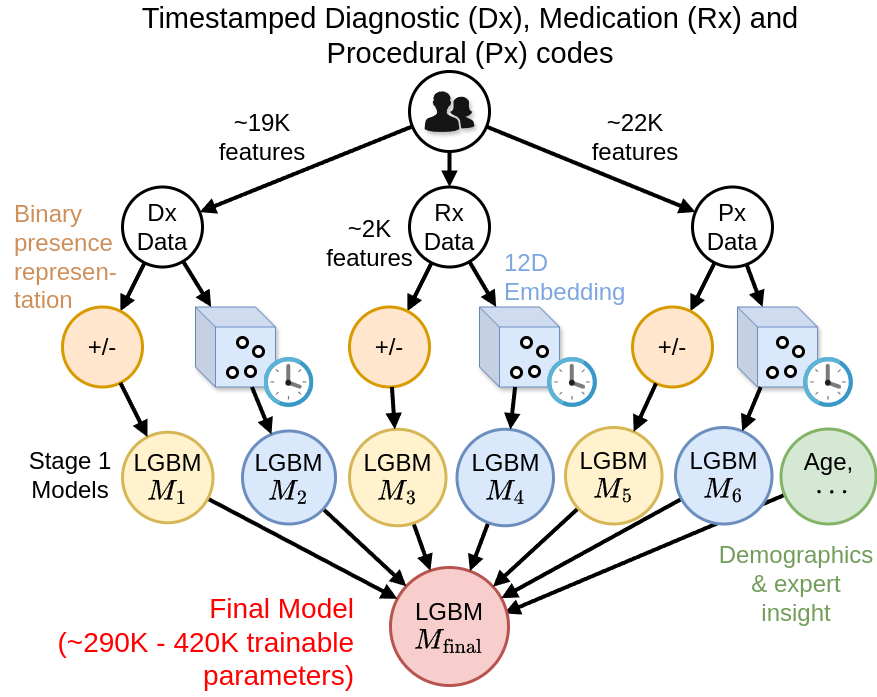
\includegraphics[width=4.1in]{Figures/zcorscheme1}

  \vspace{-10pt}
  
  \captionN{\textbf{\zcor architecture.} Combining binary presensce features of over 43K codes with a custom 12 dimensional embedding of Odds ratios of 44K codes given a well-defined target disease phenotype, with a stacked  LGBM network, yielding a final model with less than half a million trainable parameters. The emebedding can incorporate longitudinal information, resulting in a scheme that takes advantage of known AI strategies, longitudinal patterns, custom feature engineering, and expert insight into disease pathobiology.}\label{figarchitecture}
\end{wrapfigure}
\zcor is a general algorithm to predict future clinical documentation of any well-defined target
condition or composite endpoint in an individual patient's Electronic Health Record (EHR), where the target is specified by a pre-defined set of ICD-10
(and related) codes. The overall model architecture is illustrated in Figure~\ref{figarchitecture}.

\paragraph*{Prediction Task }

For each patient \( x \), a screening index point \( t_0 \) is defined, and the model estimates the risk of a  target event;  typically the first occurrence. Separate models estimate the risk of occurrence at different prediction horizons, $e.g.$  1 week, 1 month or 6 months in future post-\( t_0 \).

\paragraph*{Data Source} Training data are drawn from large EHR and claims databases, $e.g.$ the Merative MarketScan claims dataset~\cite{hansen2017truven} (with adequate train/validation split), and comprises diagnostic (Dx), procedural (Px), and pharmacy (Rx) codes. The performance results reported for the different scenarios are obtained for out-of-sample held-back data from the database.  Patients are stratified by sex, and possibly also by age when it is relevant. \zcor is trained on cohorts which exclude patients who do not have a pre-specified length of visibility in the datsbase, typically $1-2$ years. Controls are age-matched, target-code-free, with a pre-specified length (typically $\geqq 3 $ years) over which they are visible in the datbase being used.

\paragraph*{Timeline and Observation Window} For cases, the screening index point is set  prior to the first target code by the length of the prediction horizon. For controls, the index point is generally  2 years before their final record to ensure target-free follow-up of two years after screening index point. Thus, the observation window (the data used for training for each patient) spans at least 1 year  before the index point. These values can be altered to suite a particular problem.

\begin{table}[!ht]
\centering
\fontsize{9}{10}\selectfont

\caption{ICD-10 codes used to define the case cohort}
\label{table_target}

\begin{tabular}{|
>{\raggedright\arraybackslash}L{1.6in}|
>{\raggedright\arraybackslash}L{4.8in}|
}
\hline
\rowcolor{black!30}
Condition & Codes \\
\hline

Suicidal ideations & R45.851 \\
\hline

Suicide attempts & T14.91 T14.91XA T14.91XD T14.91XS \\
\hline

Intentional self-harm &
X71 X71.0XXA X71.0XXD X71.0XXS X71.1XXA X71.1XXD X71.1XXS X71.2XXA X71.2XXD X71.2XXS X71.3XXA X71.3XXD X71.3XXS X71.8XXA X71.8XXD X71.8XXS X71.9XXA X71.9XXD X71.9XXS X72 X72.XXXA X72.XXXD X72.XXXS X73 X73.0XXA X73.0XXD X73.0XXS X73.1XXA X73.1XXD X73.1XXS X73.2XXA X73.2XXD X73.2XXS X73.8XXA X73.8XXD X73.8XXS X73.9XXA X73.9XXD X73.9XXS X74 X74.01XA X74.01XD X74.01XS X74.02XA X74.02XD X74.02XS X74.09XA X74.09XD X74.09XS X74.8XXA X74.8XXD X74.8XXS X74.9XXA X74.9XXD X74.9XXS X75 X75.XXXA X75.XXXD X75.XXXS X76 X76.XXXA X76.XXXD X76.XXXS X77 X77.0XXA X77.0XXD X77.0XXS X77.1XXA X77.1XXD X77.1XXS X77.2XXA X77.2XXD X77.2XXS X77.3XXA X77.3XXD X77.3XXS X77.8XXA X77.8XXD X77.8XXS X77.9XXA X77.9XXD X77.9XXS X78 X78.0XXA X78.0XXD X78.0XXS X78.1XXA X78.1XXD X78.1XXS X78.2XXA X78.2XXD X78.2XXS X78.8XXA X78.8XXD X78.8XXS X78.9XXA X78.9XXD X78.9XXS X79 X79.XXXA X79.XXXD X79.XXXS X80 X80.XXXA X80.XXXD X80.XXXS X81 X81.0XXA X81.0XXD X81.0XXS X81.1XXA X81.1XXD X81.1XXS X81.8XXA X81.8XXD X81.8XXS X82 X82.0XXA X82.0XXD X82.0XXS X82.1XXA X82.1XXD X82.1XXS X82.2XXA X82.2XXD X82.2XXS X82.8XXA X82.8XXD X82.8XXS X83 X83.0XXA X83.0XXD X83.0XXS X83.1XXA X83.1XXD X83.1XXS X83.2XXA X83.2XXD X83.2XXS X83.8XXA X83.8XXD X83.8XXS \\
\hline

\end{tabular}
\end{table}

\begin{table}[!ht]
\centering
\fontsize{9}{10}\selectfont

\caption{Feature and Parameter Counts by Model}
\label{table_MODEL_NUMBERS}

\begin{tabular}{|
>{\raggedright\arraybackslash}L{0.90in}|
>{\raggedleft\arraybackslash}L{0.49in}|
>{\raggedleft\arraybackslash}L{0.505in}|
>{\raggedleft\arraybackslash}L{0.49in}|
>{\raggedleft\arraybackslash}L{0.505in}|
>{\raggedleft\arraybackslash}L{0.49in}|
>{\raggedleft\arraybackslash}L{0.505in}|
>{\raggedleft\arraybackslash}L{0.505in}|
>{\raggedleft\arraybackslash}L{0.49in}
|}
\hline
\rowcolor{black!30}
Model &
\# DX Features & \# DX Trainable Parameters &
\# RX Features & \# RX Trainable Parameters &
\# PROC Features & \# PROC Trainable Parameters &
\# Total Trainable Parameters & \# Total Features \\
\hline

Males, 25--50   & 19,496 & 134,556 & 1,940 & 116,938 & 21,225 & 141,514 & 393,008 & 42,662 \\
\hline
Females, 25--50 & 20,578 & 201,655 & 2,020 & 180,761 & 22,081 & 225,930 & 608,346 & 44,680 \\
\hline
Males, 50--75   & 19,042 & 94,322  & 1,992 & 86,716  & 22,246 & 101,299 & 282,337 & 43,281 \\
\hline
Females, 50--75 & 19,553 & 118,395 & 2,035 & 108,893 & 22,561 & 130,015 & 357,303 & 44,150 \\
\hline

\end{tabular}
\end{table}

 

\paragraph*{Feature Engineering}
Denoting the  medical history $H_j(x)$  for each patient $x$ is denoted as: 
\cgather{
\forall j \in \left  \{Dx,Rx,Px \right \}, \ W^j(x) = \left \{ (c_1^j,t_1^j), \cdots, (c_i^j,t_i^j), \cdots, (c_r^j,t_r^j) \right \}, c_i^j \in C_j
}%
where $t_i^j$ are logging time points for the recorded codes, and $C_j$ are set of valid codes for each channel. We map each patient's medical history to representations, namely the binary presense feature vector, and the odds-ratio embedding vector described next.
%% \begin{itemize}
%% \item \textbf{Presence features:} Binary indicators
%% \cgather{
%%  \forall j \in \left  \{Dx,Rx,Px \right \}, \ x_j^{\text{presence}} = \left  \{  \mathbb{I}\left (c  \in H_j(x)\right ): c \in \mathcal{C}_{j} \right \}
%%   }
%%   where \( \mathcal{C}_{j} \) is the set of all distinct codes in channel \( j \), and $\mathbb{I}$ is the indicator function.
%%     \item \textbf{Odds-ratio sequence embeddings:} For each code \( c \in \mathcal{C}_{j}\), we compute the odds-ratio disctionary:
%%     \cgather{
%%   \forall c \in \mathcal{C}_{j},  \ \text{OR}_j(c) =  \frac{P(\exists t \text{ s.t. } (c,t) \in W^j(y) \vert y \in \textbf{cases})}{P(\exists t  \text{ s.t. }(c,t) \in W^j(z) \vert z \in \textbf{controls})}
%%     }%
%%     We then map patient $x$ to a 12-dimensional embedding via functions \( \mathcal{A}_k \):
%%     \cgather{
%%   \forall j \in \left  \{Dx,Rx,Px \right \}, \  x^{\text{OR}}_j = \left \{ \mathcal{A}_k \left( \left\{ \text{OR}_j(c) \vert \exists t \text{ s.t. } (c,t) \in W^j(x) \right\} \right), \quad k = 1,\dots,12 \right \}
%%     }
%%     These embedding functions range from statistical measures such as variance corrected mean, range and other possibly sequence characteristic reflecting longitudinal patterns.
%% \end{itemize}

\paragraph*{Prescription Drug Coding}
 
Prescription drug (RX) codes in our primary (National) dataset are provided in the National Drug Code (NDC) format~\cite{FDA_NDC}, which is designed to facilitate the identification and commercial distribution of pharmaceuticals. This coding system, as well as the widely adopted RxNorm~\cite{NLM_RxNorm} emphasizes product-specific and manufacturer details of the generic drugs rather than their therapeutic classification and characteristics, thus hindering its use for EHR data analysis.

%% \begin{wrapfigure}[12]{r}{3in}

%%   \vspace{0pt}
  
%%   \includegraphics[width=3in]{Figures/RX_CODE_EXAMPLE.png}

%%   \captionN{NDC drug naming convention}\label{figcode}
%%   \end{wrapfigure}
To facilitate the analysis of prescriptions according to their therapeutic effect, we developed a custom NDC-compatible coding scheme to convert all RX codes in the used datasets. This system, analogous to \ICD for diagnostic codes, progressively details therapeutic information of a generic drug with each successive character in the code. Each RX code begins with an ``rx'' prefix to enhance readability and facilitate parsing. This is followed by three alphanumeric characters encoding, respectively, the Therapeutic Group, Therapeutic Class, and Therapeutic Subclass, latter derived from the Therapeutic Class column in the RED BOOK. In cases where any of these attributes are missing or listed as NEC (i.e., not elsewhere classifiable), we use the placeholder character ``X''. Finally, to identify a specific generic drug, we append a numeric identifier indicating its order within the set of drugs sharing the same initial five-letter therapeutic code.% (see Figure~\ref{figcode}e for the example of generic drug coding). %Information on NDC codes and the corresponding therapeutic attributes of the generic drugs they represent is typically sourced from the Micromedex RED BOOK\textsuperscript{\textcopyright}~\cite{Merative_RedBook}. 

\paragraph*{Code Presence Embedding Vectors}
For each EHR data channel $j \in D$, we define a binary presence embedding based on the patient observation window $W^j(x)$. Let $C^j$ denote the set of all distinct codes observed across the embedding inference set, augmented with hierarchical code prefixes to enable generalization across varying code granularities.

Specifically, we include for each code $c \in C^j$ its prefixes according to the following scheme:
\begin{itemize}
    \item DX: prefixes of length 1, 2, 3, 5 and 6,
    \item RX: prefixes of length 3, 4, 5, and 8,
    \item PROC: prefixes of length 1, 2, 3, 4, and 5.
\end{itemize}

We define the augmented code set $\mathcal{C}^j$ for channel $j$ as:
\[
\mathcal{C}^j = \left\{ \text{all codes and specified-length prefixes observed in Code Inference Set} \right\}
\]

Let $\mathcal{O}^j(x)$ be the set of codes and code prefixes present in the observation window $W^j(x)$ for patient $x$. Then, the presence vector $x^{\text{presence}}_j \in \{0, 1\}^{|\mathcal{C}^j|}$ is defined elementwise as:

\begin{equation}
\forall c_i \in \mathcal{C}^j, \quad x^{\text{presence}}_{j,i}(x) =
\begin{cases}
1, & \text{if } c_i \in \mathcal{O}^j(x) \\
0, & \text{otherwise}
\end{cases}
\end{equation}

In total, the number of codes and code prefixes we track is $>20,000$ for $D_X$ channel, $>2000$ for $R_X$ channel, and $>17,000$ for $P_X$ channel. 
%See Table~\ref{SI-tab_N_PRESENCE_CODES} for the total number of codes and prefix-based aggregations used in each presence model. The resulting binary vectors serve as input to the gradient boosting classifiers for each EHR channel.

\paragraph*{Odds Ratio Embedding Vectors}

For each code $c \in C^j$, in each data channel $j \in D$, we compute the dictionary of cubed odds ratios based on patients from the Code Inference Set:

\begin{equation}
\forall c \in C^j, \quad \text{OR}^j(c) = \left( \frac{\mathbb{P}(\exists t \text{ s.t. } (c, t) \in W^j(y) \mid y \in \text{cases})}{\mathbb{P}(\exists t \text{ s.t. } (c, t) \in W^j(z) \mid z \in \text{controls})} \right)^3
\end{equation}

Then we compute odds ratios for all codes in the patients' observation windows:

\begin{equation}
\forall j \in D, \quad x^{\text{OR}}_j = \left\{ \text{OR}^j(c), \ c \in W^j(x) \right\}
\end{equation}

and finally map the computed odds ratios of each patient $x$ to a 12-dimensional embedding via aggregation functions $\mathcal{A}_k$

\begin{equation}
\forall j \in D, \quad x^{\text{OR\_embedding}}_j = \left\{ \mathcal{A}_k\left(x^{\text{OR}}_j \right) \;\middle|\; k = 1, \ldots, 12 \right\}
\end{equation}
%Table~\ref{tab_OR_AGGREGATIONS} enumerates for the complete list of aggregation functions $\mathcal{A}_k$.

\section*{Model Architecture}
\zcor is a stacked ensemble of LightGBM models~\cite{ke2017lightgbm} with $6$ base classifiers (Fig.~\ref{figarchitecture}):
\cgather{
\forall j \in \left  \{Dx,Rx,Px \right \},   k \in \{\text{presence}, \text{OR}\}, \wp_{j,k}(x) = f^{\text{base}}_{j,k}(x_j^k)
}%
These six risk outputs are used to train a final LGBM classifier, which also takes  as input patient age, and other demographic characteristics (referred to as the set $\text{CHAR}$), to estimate the final \zcor risk $\wp$:
\cgather{
\wp(x) = f^{\text{final}}\left (\left \{ \rho_{j,k}(x):\forall j \in \left  \{Dx,Rx,Px \right \},   k \in \{\text{presence}, \text{OR}\}  \right  \}\cup \left \{v_i(x): v_i \in \text{CHAR} \right \} \right )
}%
\paragraph*{Training} The  set of eligible patients from the database under consideration  is split typically 66\% - 34\% for training and validation. The training set is further split 60/40 for computing odds ratios and training the final LGBM model.
We consider almost all unique  diagnostic, medication and procedural codes as feature inputs, stratified into the Dx, Rx and Px channels, using in total 43,609 and 42,858 feature inputs respectively for the models corresponding to  50+ (older patients)  and 25-50 (younger patients) age groups. The overall \zcor model has sufficient capacity for the EHR data at-hand, and we can measure the model  complexity as the number of independent (or trainable) parameters (See Table~\ref{table_MODEL_NUMBERS}, number of trainable parameters for the problems targeted here range betwee 35,748 - 68,320). 

Gradient boosting machines, which are the conceptual foundations for LighGBMs,  are decision-tree ensembles, and the \zcor framework, with its stacked network of LGBMs, realizes a non-linear classifier that optimizes the contribution of different EHR data modalities, while making sure the model architecture is not too unconstrained.  In particular, \zcor  avoids off-the-shelf embeddings ($e.g.$, transformer architectures) in favor of a custom 12D embedding of odd-ratios of Dx, Rx and Px codes. Such  neural models  use hundreds of millions of parameters (2 orders of magnitude more  in this application), \zcor’s more limited parameter count ($<0.5$M) enables  more efficient training, faster inference, better generalization in sparse, weakly labeled data, and robustness to population shifts and health system idiosyncrasies.




\section*{Statistical Analyses, Models and Sufficiency of Sample Size} The \zcor performance is measured using standard ML measures such as AUC, likelihood ratios, PPV, NPV and others, as has been demonstrated in several past studies~\cite{onishchenko2021reduced,onishchenko2022screening,JAHA2022}. % The evaluation of the \zcorp workflow will involve statistical estimation of several measures outlined in later section on implementation science frameworks. 
%
Our sample size needs to be adequate when we train and evaluate \zcor . Here the sample size sufficiency question relates to if we would have sufficient number of patients to acceptably bound the uncertainty of our predictions, to confidently validate the tool. The CI for the  AUC are calculated using  the  equivalence with the Mann-Whitney U statistic~\cite{birnbaum1957bounds,mann1947test,wilcoxon1992individual}. We 
carry out bootstrapped runs over randomly selected sub-cohorts   estimating the empirical distribution of AUC over these runs; in the example shown, the mean AUCs obtained by this approach were within $\pm 2\%$ of the U statistic estimate for sufficiently large sub-cohorts. The CI for specificity and sensitivity are computed via  the asymptotic method for single proportions~\cite{newcombe1994confidence} (the Wald Method). CI for the remaining metrics (PPV, likelihood ratios) are computed from the extremal values of the CI for specificity and sensitivity. We also compute p-values for the null hypotheses that \pcor performance is different from a corresponding baseline for the same sex and dataset using a small fixed set of risk factors (presence or absence of specific mental disorders), using Dantzig's upper bound on AUC variance~\cite{birnbaum2020use,vandantzig1951consistency}.
 In the example shown, these considerations suggest an estimated minimum sample size 
 of  1435 (1 week horizon) -  1988 (6 month horizon) 
 to yield AUC estimates with a maximum error of $<\pm 0.02$ with 95\% probability, assuming a $10\%$ target prevalence. Generally, this is a highly realizable goal given the patient numbers we typically encounter in a hospital system.


 %% \section*{Attribution: The $\SPOR$ }
%% Large-scale observational datasets — spanning genomics biobanks, administrative claims, and electronic health records (EHR) — increasingly drive scientific discovery and risk modeling. Odds ratios (ORs) and related effect-size estimates remain the dominant tools for summarizing exposure-outcome associations. Yet as cohort sizes reach hundreds of thousands or millions, naive OR analysis breaks down: effect sizes inflate, $p$-values vanish, and nearly all features appear statistically significant, even when no true association exists.

%% This pathology reflects two structural vulnerabilities of large observational studies:
%% \begin{enumerate}
%%     \item \textbf{Label Noise:} Case/control labels are often derived from imperfect sources such as diagnostic codes or weak classifiers, introducing systematic misclassification~\cite{halpern2016electronic}.
%%     \item \textbf{Large Sample Size Effects:} As $n \to \infty$,  variance estimates collapse, magnifying even trivial fluctuations or structural biases, yielding spurious discoveries~\cite{greenland1988sensitivity,miguel2023causal}.
%% \end{enumerate}

%% In randomized trials, ORs approximate causal contrasts under minimal assumptions. In contrast, observational settings lack experimental control; naive OR computations applied directly to raw exposure-outcome tables, without adjustment for label noise or structural confounding, produce exaggerated significance that worsens with scale.

%% Post-hoc attribution methods such as SHAP and LIME~\cite{lundberg17shap} offer model-agnostic feature importance scores, but inherit related limitations: they remain artificially stable under weak, non-predictive models, overlook interaction-driven effects, and fail to correct for misclassification or instability~\cite{slack2020fooling}.

%% Existing corrections for OR bias primarily target small-sample misclassification adjustment~\cite{greenland1988sensitivity}, or require external gold-standard validation cohorts, which are rarely available at scale.

%% We introduce the \emph{lambda-Odds Ratio ($\SPOR$)}, a model-informed, asymptotically faithful method for effect-size estimation and feature attribution tailored to large, noisy observational datasets. 
%% $\SPOR$ differs from classical OR estimation:
%% \begin{enumerate}
%%     \item Individuals are stratified by calibrated model-predicted risk, forming empirical high- and low-risk cohorts.
%%     \item Exposure odds contrasts are computed across these strata, rather than from unstratified marginal tables.
%%     \item A ridge-regularized inversion corrects for outcome misclassification and ensures numerical stability, even under near-degenerate class distributions.
%% \end{enumerate}

%% We consider retrospective observational studies where binary case/control labels \( \tilde{Y} \in \{0,1\} \) are derived from imperfect classifiers or noisy diagnostic records (e.g., EHR-derived phenotypes), and exposure status \( X \in \{0,1\} \) is assumed to be known without error. Let the observed (noisy) 2-by-2 contingency table be
%% \cgather{
%% \tilde{T} = \begin{bmatrix}
%% \tilde{a} & \tilde{b} \\
%% \tilde{c} & \tilde{d}
%% \end{bmatrix},
%% }
%% where \( \tilde{a} \) denotes the count of individuals with \( X=1 \) and \( \tilde{Y}=1 \), and so on. These observed labels are subject to misclassification governed by sensitivity \( p = \mathbb{P}(\tilde{Y}=1 \mid Y=1) \) and specificity \( q = \mathbb{P}(\tilde{Y}=0 \mid Y=0) \), where \( Y \) denotes the true latent label.

%% The misclassification process is represented by the stochastic matrix
%% \cgather{
%% K = \begin{bmatrix}
%% p & 1 - p \\
%% 1 - q & q
%% \end{bmatrix},
%% }
%% so that the observed counts satisfy, in expectation,
%% \cgather{
%% \tilde{T} = T K^\top,
%% }
%% where \( T \) is the true (unknown) count matrix under perfect case/control assignment.

%% \paragraph*{Ill-posed Inversion and the Need for Regularization}\
%% Inversion of $K^\top$ to estimate \( T \) via \( T = \tilde{T} (K^\top)^{-1} \) can result in infeasible solutions where the recovered cell counts are negative or numerically unstable, particularly when \( K \) is nearly singular or \( p + q \approx 1 \). To address this, we adopt a ridge-regularized inverse:
%% \cgather{
%% T^{(\lambda)} \triangleq \tilde{T} (K^\top + \lambda I)^{-1},
%% }
%% where \( \lambda > 0 \) is chosen to ensure all entries of \( T^{(\lambda)} \) remain nonnegative and greater than a small threshold \( \epsilon \), preserving interpretability as approximate counts. The minimal such \( \lambda \), if it exists, defines our feasible correction. The regularized corrected contingency table is denoted
%% \cgather{
%% T^{(\lambda)} = \begin{bmatrix}
%% a & b \\
%% c & d
%% \end{bmatrix},
%% }
%% and the corrected log-odds ratio is
%% \cgather{\logor^{(\lambda)} = \log\left( \frac{a d}{b c} \right).
%% }
%% We estimate the standard error using the delta method, optionally incorporating the uncertainty in \( p, q \) (from validation data) via an analytic extra-variance term.

%% This framework generalizes classical odds ratio inference by explicitly modeling outcome misclassification and providing a consistent correction even when label quality varies or depends on classifier thresholds.

%% \begin{table}[t]
%% \centering
%% \small
%% \caption{
%%   \textbf{Odds Ratios Aggregations} 
%% }\label{tab_OR_AGGREGATIONS}
%% \begin{tabular}{R{2in} L{4in} } \hline
%% \textbf{Aggregation Name} & \textbf{Formula} \\ \hline
%% \textrm{mean\_or} & $\text{mean}(r), \ \forall r \in \ x^{\text{OR}}_j$ \\ 
%% {max\_or} & $\text{max}(r), \ \forall r \in \ x^{\text{OR}}_j$ \\ 
%% {sum\_or} & $\text{sum}(r), \ \forall r \in \ x^{\text{OR}}_j$ \\ 
%% {std\_or} & $\text{standard\_deviation}(r), \ \forall r \in \ x^{\text{OR}}_j$ \\ 
%% {range\_or} & $\max(r) - \min(r), \ \forall r \in \ x^{\text{OR}}_j$ \\ 
%% {geomean\_or} & $\text{geometric\_mean}\left( [r \text{ if } r \neq 0 \text{ else } 10^{-7}], \ \forall r \in \ x^{\text{OR}}_j \right)$ \\ 
%% {variation\_or} & $\text{variation}\left( [r \text{ if } r \neq 0 \text{ else } 10], \ \forall r \in \ x^{\text{OR}}_j \right)$ \\ 
%% {meanstd\_or} & $\operatorname{mean\_or} \times \operatorname{std\_or}$ \\ 
%% {meanrng\_or} & $\operatorname{mean\_or} \times \operatorname{range\_or}$ \\ 
%% {meanstd\_sq\_or} & $\operatorname{mean\_or}^{\operatorname{std\_or}}$ \\ 
%% {geomeanrng\_or} & $\operatorname{geomean\_or} \times \operatorname{range\_or}$ \\ 
%% {geomean\_sq\_sum} & $\sqrt{\operatorname{geomean\_or}^{\operatorname{sum\_or}}}$ \\ \hline
%% \end{tabular}
%% \end{table}

%% \paragraph*{Interpretation}

%% This approach defines a class of corrected log-odds ratio estimators indexed by \( \lambda \), each balancing fidelity to the noisy data against feasibility under misclassification uncertainty. In the limit \( \lambda \to 0 \), the estimator recovers the unregularized inverse, which may become undefined or yield negative entries. The practical estimator uses the smallest \( \lambda \) such that all recovered counts exceed a small threshold \( \epsilon > 0 \), typically \( \epsilon \in [0.1, 1] \).

%% This formulation enables consistent odds ratio estimation in large-scale electronic health record (EHR) studies, where label noise is prevalent and direct validation of every case/control label is infeasible.


%% \paragraph*{$\SPOR$ Variance Estimation}
%% Under the assumption of independent cell counts, the classical variance of the log-odds ratio is
%% \cgather{
%% \mathrm{Var}_{\text{naive}}(\logor) = \frac{1}{a} + \frac{1}{b} + \frac{1}{c} + \frac{1}{d}.
%% }%
%% However, when the table \( T^{(\lambda)} \) is obtained via inversion from noisy labels, additional uncertainty arises from the estimation of the misclassification rates \( p \) and \( q \). Let \( n_{\text{val}} \) denote the size of the validation cohort used to estimate \( p \) and \( q \), assumed independent of the main study population. Define the extra-variance component via the delta method as
%% \cgather{
%% \mathrm{Var}_{\text{extra}} = \left( \left( \frac{1-q}{(p + q - 1)^2} \right)^2 \frac{p(1-p)}{n_{\text{val}}} \right. + \left. \left( \frac{1-p}{(p + q - 1)^2} \right)^2 \frac{q(1-q)}{n_{\text{val}}} \right)
%% }%
%% where \( n_{\text{val}} > 1  \). The total variance is given by
%% \cgather{
%% \mathrm{Var}_{\text{total}}(\logor) =\mathrm{Var}_{\text{naive}} +  \mathrm{Var}_{\text{extra}}.
%% }%
%% The corrected Wald statistic is: $
%% Z = \frac{\logor^{(\lambda)}}{\sqrt{\mathrm{Var}_{\text{total}}}},
%% $, with a  two-sided p-value obtained from the standard normal tail: $p_{\text{two}} = 2 \Phi(-|Z|)$, with the \( (1 - \alpha) \) confidence interval:
%% \cgathers{
%% \Big [ \logor^{(\lambda)} - z_{\alpha/2}  \sqrt{\mathrm{Var}_{\text{total}}},
%%        \logor^{(\lambda)} + z_{\alpha/2}  \sqrt{\mathrm{Var}_{\text{total}}} \Big ]
%%      }%
%% using \( z_{\alpha/2} \) as the critical value from the standard normal distribution.  

